\documentclass[journal=jcisd8,manuscript=suppinfo]{achemso}

\usepackage{amsmath,amssymb}
\usepackage{graphicx}
\usepackage{booktabs}
\usepackage{multirow}
\usepackage{siunitx}
\usepackage[dvipsnames]{xcolor}

\title{Supporting Information: When Do Simple Models Win? Machine Learning Architectures for UV Absorption Prediction and Insights for General Molecular Property Prediction}

\author{Umesh Arampath}
\email{uarampath@mwbioprocessing.com}
\affiliation{Department of Mathematics, University of Iowa, Iowa City, USA}
\alsoaffiliation{Midwest Bioprocessing Center, Illinois, USA}

\author{Bryant Pero}
\affiliation{Midwest Bioprocessing Center, Illinois, USA}

\author{David Stewart}
\affiliation{Department of Mathematics, University of Iowa, Iowa City, USA}

\author{David Demirjian}
\affiliation{Midwest Bioprocessing Center, Illinois, USA}

\begin{document}

\section{Per-Fold Cross-Validation Results}
\label{sec:perfold}

Tables~\ref{tab:perfold_rf}--\ref{tab:perfold_chemberta} present per-fold results for all five model families on the primary Joung+Beard dataset (stratified 5-fold CV, 64/16/20 split).

\begin{table}[htbp]
\centering
\caption{Per-fold RF + Morgan FP results (tuned, with solvent).}
\label{tab:perfold_rf}
\begin{tabular}{ccccc}
\toprule
\textbf{Fold} & \textbf{RMSE (nm)} & \textbf{MAE (nm)} & $\boldsymbol{R^2}$ & \textbf{Pearson $r$} \\
\midrule
0 & 32.02 & 15.42 & 0.907 & 0.953 \\
1 & 30.74 & 14.79 & 0.918 & 0.959 \\
2 & 28.09 & 14.47 & 0.931 & 0.965 \\
3 & 32.58 & 15.56 & 0.908 & 0.953 \\
4 & 33.25 & 15.54 & 0.905 & 0.952 \\
\midrule
\textbf{Mean $\pm$ Std} & \textbf{31.34 $\pm$ 1.82} & \textbf{15.16 $\pm$ 0.44} & \textbf{0.914 $\pm$ 0.010} & \textbf{0.956 $\pm$ 0.005} \\
\bottomrule
\end{tabular}
\end{table}

\begin{table}[htbp]
\centering
\caption{Per-fold BiGRU + Solvent results (v2).}
\label{tab:perfold_bigru}
\begin{tabular}{ccccc}
\toprule
\textbf{Fold} & \textbf{RMSE (nm)} & \textbf{MAE (nm)} & $\boldsymbol{R^2}$ & \textbf{Pearson $r$} \\
\midrule
0 & 35.23 & 20.02 & 0.888 & 0.942 \\
1 & 37.33 & 20.86 & 0.879 & 0.937 \\
2 & 34.96 & 20.77 & 0.893 & 0.945 \\
3 & 37.62 & 21.51 & 0.877 & 0.937 \\
4 & 37.12 & 20.32 & 0.881 & 0.939 \\
\midrule
\textbf{Mean $\pm$ Std} & \textbf{36.45 $\pm$ 1.12} & \textbf{20.70 $\pm$ 0.51} & \textbf{0.884 $\pm$ 0.006} & \textbf{0.940 $\pm$ 0.003} \\
\bottomrule
\end{tabular}
\end{table}

\begin{table}[htbp]
\centering
\caption{Per-fold BiGRU (tuned, 3L/256u) results.}
\label{tab:perfold_bigru_tuned}
\begin{tabular}{ccccc}
\toprule
\textbf{Fold} & \textbf{RMSE (nm)} & \textbf{MAE (nm)} & $\boldsymbol{R^2}$ & \textbf{Pearson $r$} \\
\midrule
0 & 35.42 & 18.79 & 0.887 & 0.942 \\
1 & 35.51 & 17.91 & 0.890 & 0.944 \\
2 & 32.02 & 17.33 & 0.910 & 0.954 \\
3 & 35.91 & 18.76 & 0.888 & 0.943 \\
4 & 34.69 & 17.68 & 0.896 & 0.947 \\
\midrule
\textbf{Mean $\pm$ Std} & \textbf{34.71 $\pm$ 1.40} & \textbf{18.09 $\pm$ 0.59} & \textbf{0.894 $\pm$ 0.009} & \textbf{0.946 $\pm$ 0.005} \\
\bottomrule
\end{tabular}
\end{table}

\begin{table}[htbp]
\centering
\caption{Per-fold XGBoost + Morgan FP results (MSE loss, v2).}
\label{tab:perfold_xgboost}
\begin{tabular}{ccccc}
\toprule
\textbf{Fold} & \textbf{RMSE (nm)} & \textbf{MAE (nm)} & $\boldsymbol{R^2}$ & \textbf{Pearson $r$} \\
\midrule
0 & 34.55 & 20.15 & 0.892 & 0.945 \\
1 & 33.58 & 19.79 & 0.902 & 0.950 \\
2 & 30.63 & 19.31 & 0.918 & 0.959 \\
3 & 35.15 & 20.77 & 0.893 & 0.946 \\
4 & 34.58 & 20.23 & 0.897 & 0.948 \\
\midrule
\textbf{Mean $\pm$ Std} & \textbf{33.70 $\pm$ 1.61} & \textbf{20.05 $\pm$ 0.48} & \textbf{0.900 $\pm$ 0.009} & \textbf{0.950 $\pm$ 0.005} \\
\bottomrule
\end{tabular}
\end{table}

\begin{table}[htbp]
\centering
\caption{Per-fold Chemprop D-MPNN results (v2, multicomponent: solute + solvent).}
\label{tab:perfold_chemprop}
\begin{tabular}{ccccc}
\toprule
\textbf{Fold} & \textbf{RMSE (nm)} & \textbf{MAE (nm)} & $\boldsymbol{R^2}$ & \textbf{Pearson $r$} \\
\midrule
0 & 30.79 & 15.24 & 0.914 & 0.956 \\
1 & 35.40 & 19.96 & 0.891 & 0.944 \\
2 & 26.06 & 15.52 & 0.940 & 0.970 \\
3 & 32.70 & 16.03 & 0.907 & 0.953 \\
4 & 33.51 & 17.44 & 0.903 & 0.951 \\
\midrule
\textbf{Mean $\pm$ Std} & \textbf{31.69 $\pm$ 3.18} & \textbf{16.84 $\pm$ 1.74} & \textbf{0.911 $\pm$ 0.016} & \textbf{0.955 $\pm$ 0.009} \\
\bottomrule
\end{tabular}
\end{table}

\begin{table}[htbp]
\centering
\caption{Per-fold Chemprop D-MPNN results (v2, solute only, no solvent).}
\label{tab:perfold_chemprop_nosolvent}
\begin{tabular}{ccccc}
\toprule
\textbf{Fold} & \textbf{RMSE (nm)} & \textbf{MAE (nm)} & $\boldsymbol{R^2}$ & \textbf{Pearson $r$} \\
\midrule
0 & 33.37 & 15.95 & 0.899 & 0.949 \\
1 & 37.28 & 16.29 & 0.879 & 0.938 \\
2 & 29.31 & 15.88 & 0.925 & 0.962 \\
3 & 33.07 & 16.64 & 0.905 & 0.952 \\
4 & 35.88 & 17.64 & 0.889 & 0.943 \\
\midrule
\textbf{Mean $\pm$ Std} & \textbf{33.78 $\pm$ 2.73} & \textbf{16.48 $\pm$ 0.64} & \textbf{0.900 $\pm$ 0.015} & \textbf{0.949 $\pm$ 0.008} \\
\bottomrule
\end{tabular}
\end{table}

\begin{table}[htbp]
\centering
\caption{Per-fold ChemBERTa results (v2).}
\label{tab:perfold_chemberta}
\begin{tabular}{ccccc}
\toprule
\textbf{Fold} & \textbf{RMSE (nm)} & \textbf{MAE (nm)} & $\boldsymbol{R^2}$ & \textbf{Pearson $r$} \\
\midrule
0 & 49.31 & 23.88 & 0.780 & 0.899 \\
1 & 48.66 & 23.54 & 0.794 & 0.908 \\
2 & 47.70 & 23.05 & 0.801 & 0.909 \\
3 & 53.04 & 25.68 & 0.756 & 0.889 \\
4 & 53.24 & 25.39 & 0.756 & 0.890 \\
\midrule
\textbf{Mean $\pm$ Std} & \textbf{50.39 $\pm$ 2.30} & \textbf{24.31 $\pm$ 1.04} & \textbf{0.777 $\pm$ 0.019} & \textbf{0.899 $\pm$ 0.009} \\
\bottomrule
\end{tabular}
\end{table}


\section{Statistical Significance Tests}
\label{sec:significance}

Table~\ref{tab:significance} presents paired $t$-test results across the five cross-validation folds.
Most model comparisons are statistically significant at $\alpha = 0.05$ using the parametric paired $t$-test, with the notable exception of RF vs.\ Chemprop ($p = 0.77$).
With only $n = 5$ folds, the Wilcoxon signed-rank test (a non-parametric alternative) yields $p = 0.0625$ for all comparisons (the minimum achievable $p$-value when all 5 paired differences are concordant), providing strong directional evidence despite not reaching conventional significance.

\begin{table}[htbp]
\centering
\caption{Paired $t$-test results for RMSE comparisons across 5 folds.}
\label{tab:significance}
\begin{tabular}{lccc}
\toprule
\textbf{Comparison} & $\boldsymbol{t}$ & $\boldsymbol{p}$ & \textbf{Significant?} \\
\midrule
RF vs.\ Chemprop            & $0.31$ & 0.77 & No \\
RF vs.\ BiGRU              & $-7.08$ & 0.002 & Yes \\
RF vs.\ XGBoost            & $-8.94$ & 0.001 & Yes \\
RF vs.\ ChemBERTa          & $-31.0$ & $<$0.001 & Yes \\
XGBoost vs.\ BiGRU         & $-4.38$ & 0.012 & Yes \\
XGBoost vs.\ ChemBERTa     & $-21.8$ & $<$0.001 & Yes \\
BiGRU vs.\ ChemBERTa       & $-16.0$ & $<$0.001 & Yes \\
RF: solvent vs.\ no-solvent  & $-11.46$ & $<$0.001 & Yes \\
Chemprop: solvent vs.\ no-solvent & $-4.33$ & 0.012 & Yes \\
BiGRU: solvent vs.\ no-solvent & $-3.90$ & 0.018 & Yes \\
\bottomrule
\end{tabular}
\end{table}


\section{RF Hyperparameter Sensitivity}
\label{sec:rf_tuning}

The RF hyperparameter grid search evaluated 432 configurations varying the number of trees ($B \in \{100, 500, 1000\}$), maximum features per split ($\sqrt{d}$, $0.1d$, $0.3d$), maximum tree depth (None, 30, 50), minimum samples per leaf (1, 2, 5), fingerprint radius (2, 3), and fingerprint length (1024, 2048).
The search was conducted on fold~0 using the validation set for model selection.

The most influential parameter was \texttt{max\_features}: all top-10 configurations used $0.3d$ (30\% of features per split), compared to the scikit-learn default of $\sqrt{d}$ ($\approx$1.6\% of 4096 features).
This finding suggests that Morgan fingerprint features are sufficiently decorrelated that broader feature sampling per split improves performance.
The number of trees ($B$) showed diminishing returns beyond 500, and maximum depth had negligible effect (unlimited depth was optimal), indicating that the dataset does not suffer from overfitting with deep trees.


\section{BiGRU Training Curves}
\label{sec:learning_curves}

Figure~\ref{fig:learning_curves} shows the training and validation MAE curves for the BiGRU models, averaged across folds with $\pm 1$ standard deviation bands.
Both models converge within 75--125 epochs, with early stopping preventing overfitting.
The gap between training and validation curves indicates mild overfitting, consistent with the relatively small dataset size (12K training samples per fold).

\begin{figure}[htbp]
    \centering
    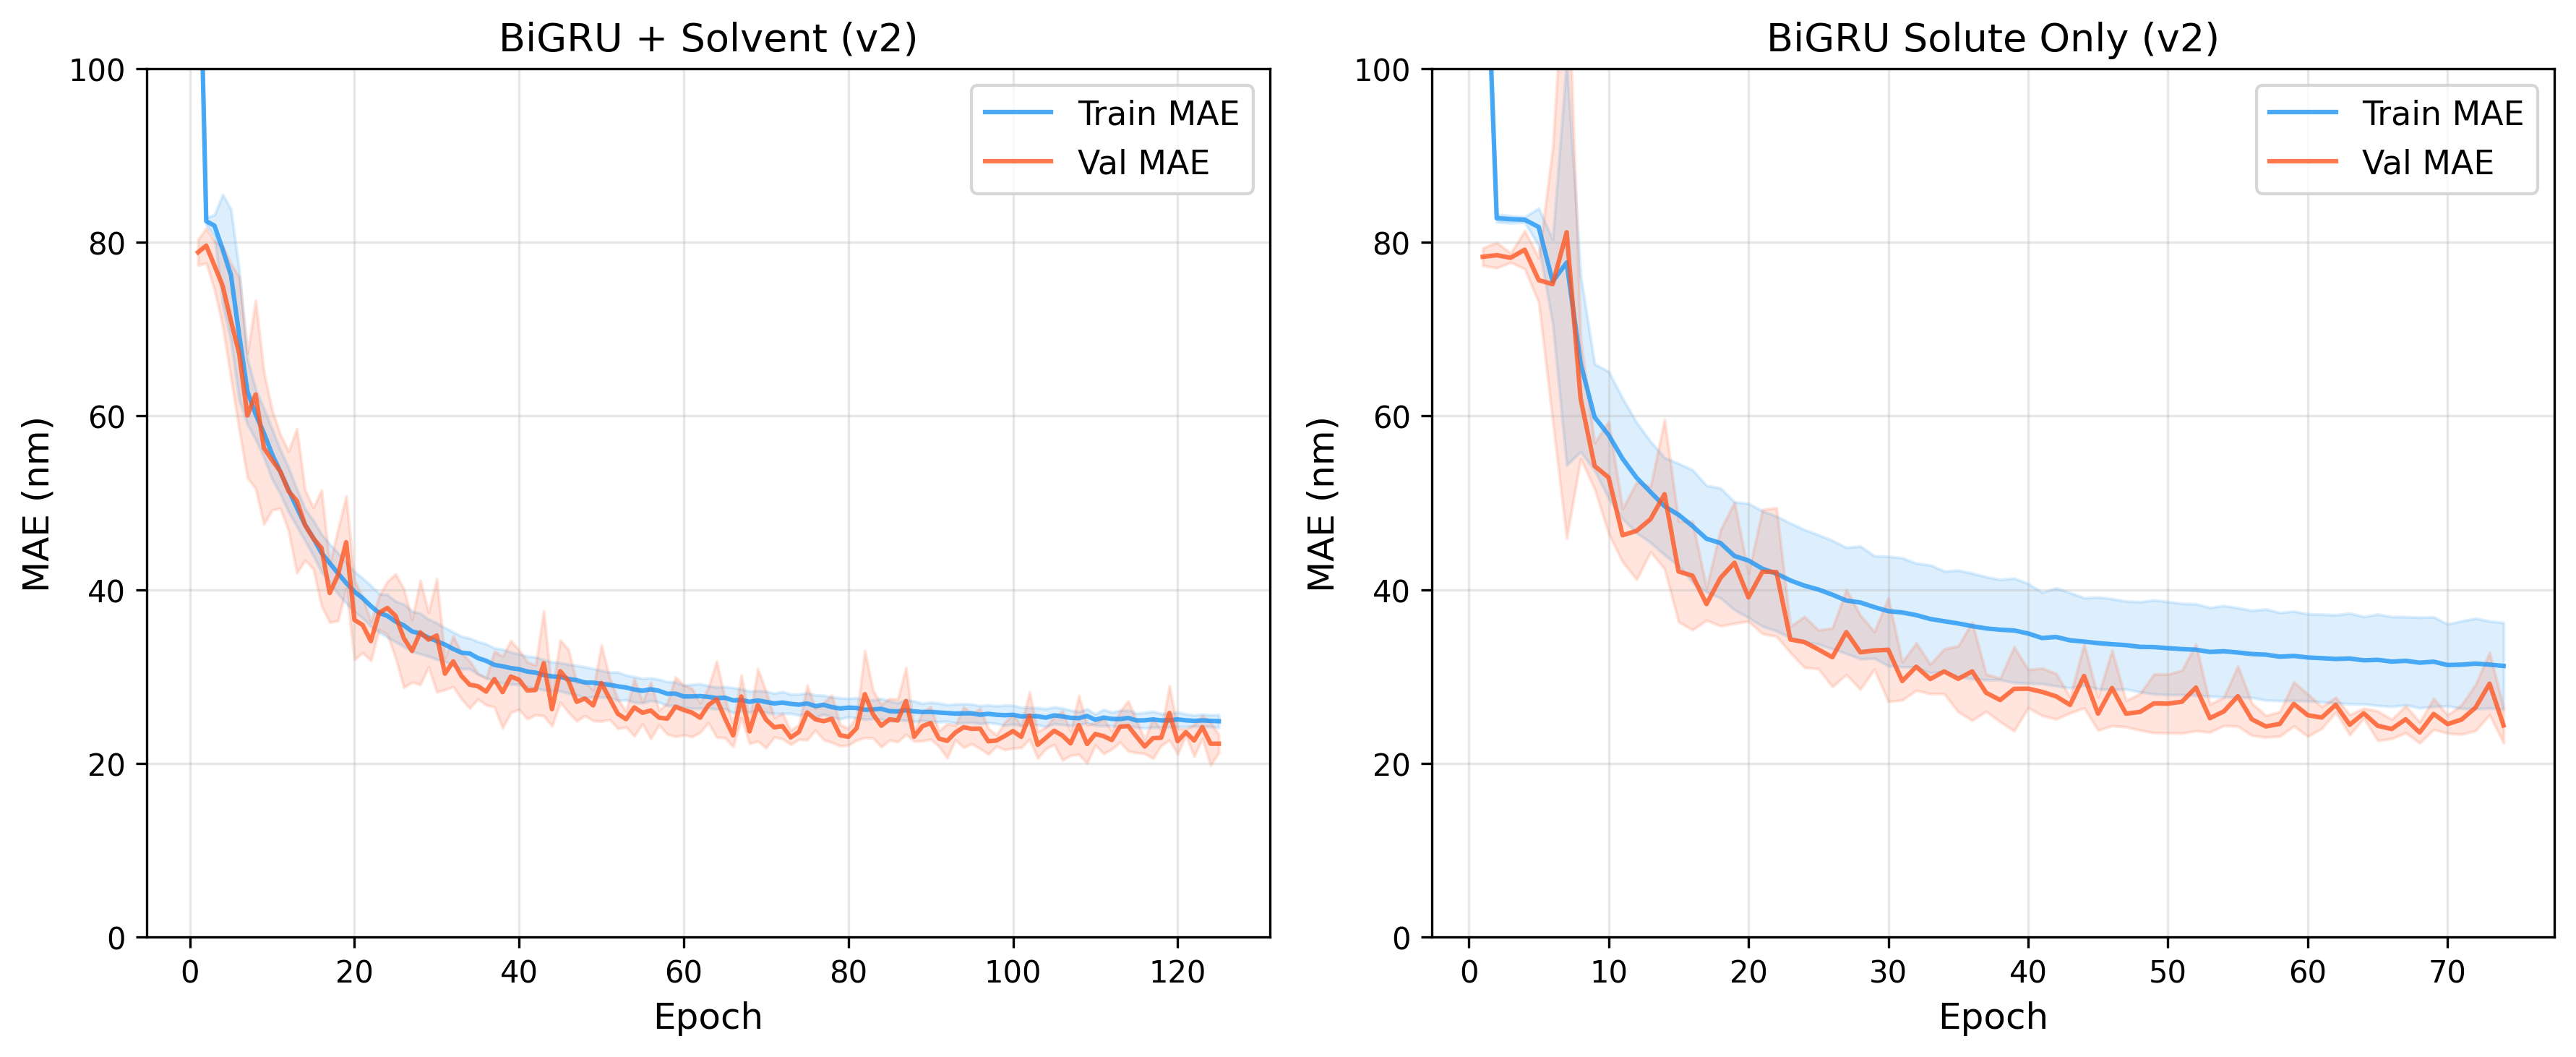
\includegraphics[width=0.9\textwidth]{results/learning_curves.png}
    \caption{BiGRU training curves showing training and validation MAE vs.\ epoch, averaged across folds. Shaded regions denote $\pm 1$ standard deviation. Left: BiGRU with solvent encoding. Right: BiGRU with solute only.}
    \label{fig:learning_curves}
\end{figure}


\section{ChemBERTa Learning Curves}
\label{sec:chemberta_curves}

Figure~\ref{fig:chemberta_curves} shows the ChemBERTa training and validation MAE curves across all five folds.
All folds converge within 40--60 epochs, with the final validation MAE plateauing around 24--26~nm.
The gap between training and validation MAE is larger than for BiGRU, consistent with ChemBERTa's 44.1M parameters being overparameterized for the $\sim$12K training samples available per fold.

\begin{figure}[htbp]
    \centering
    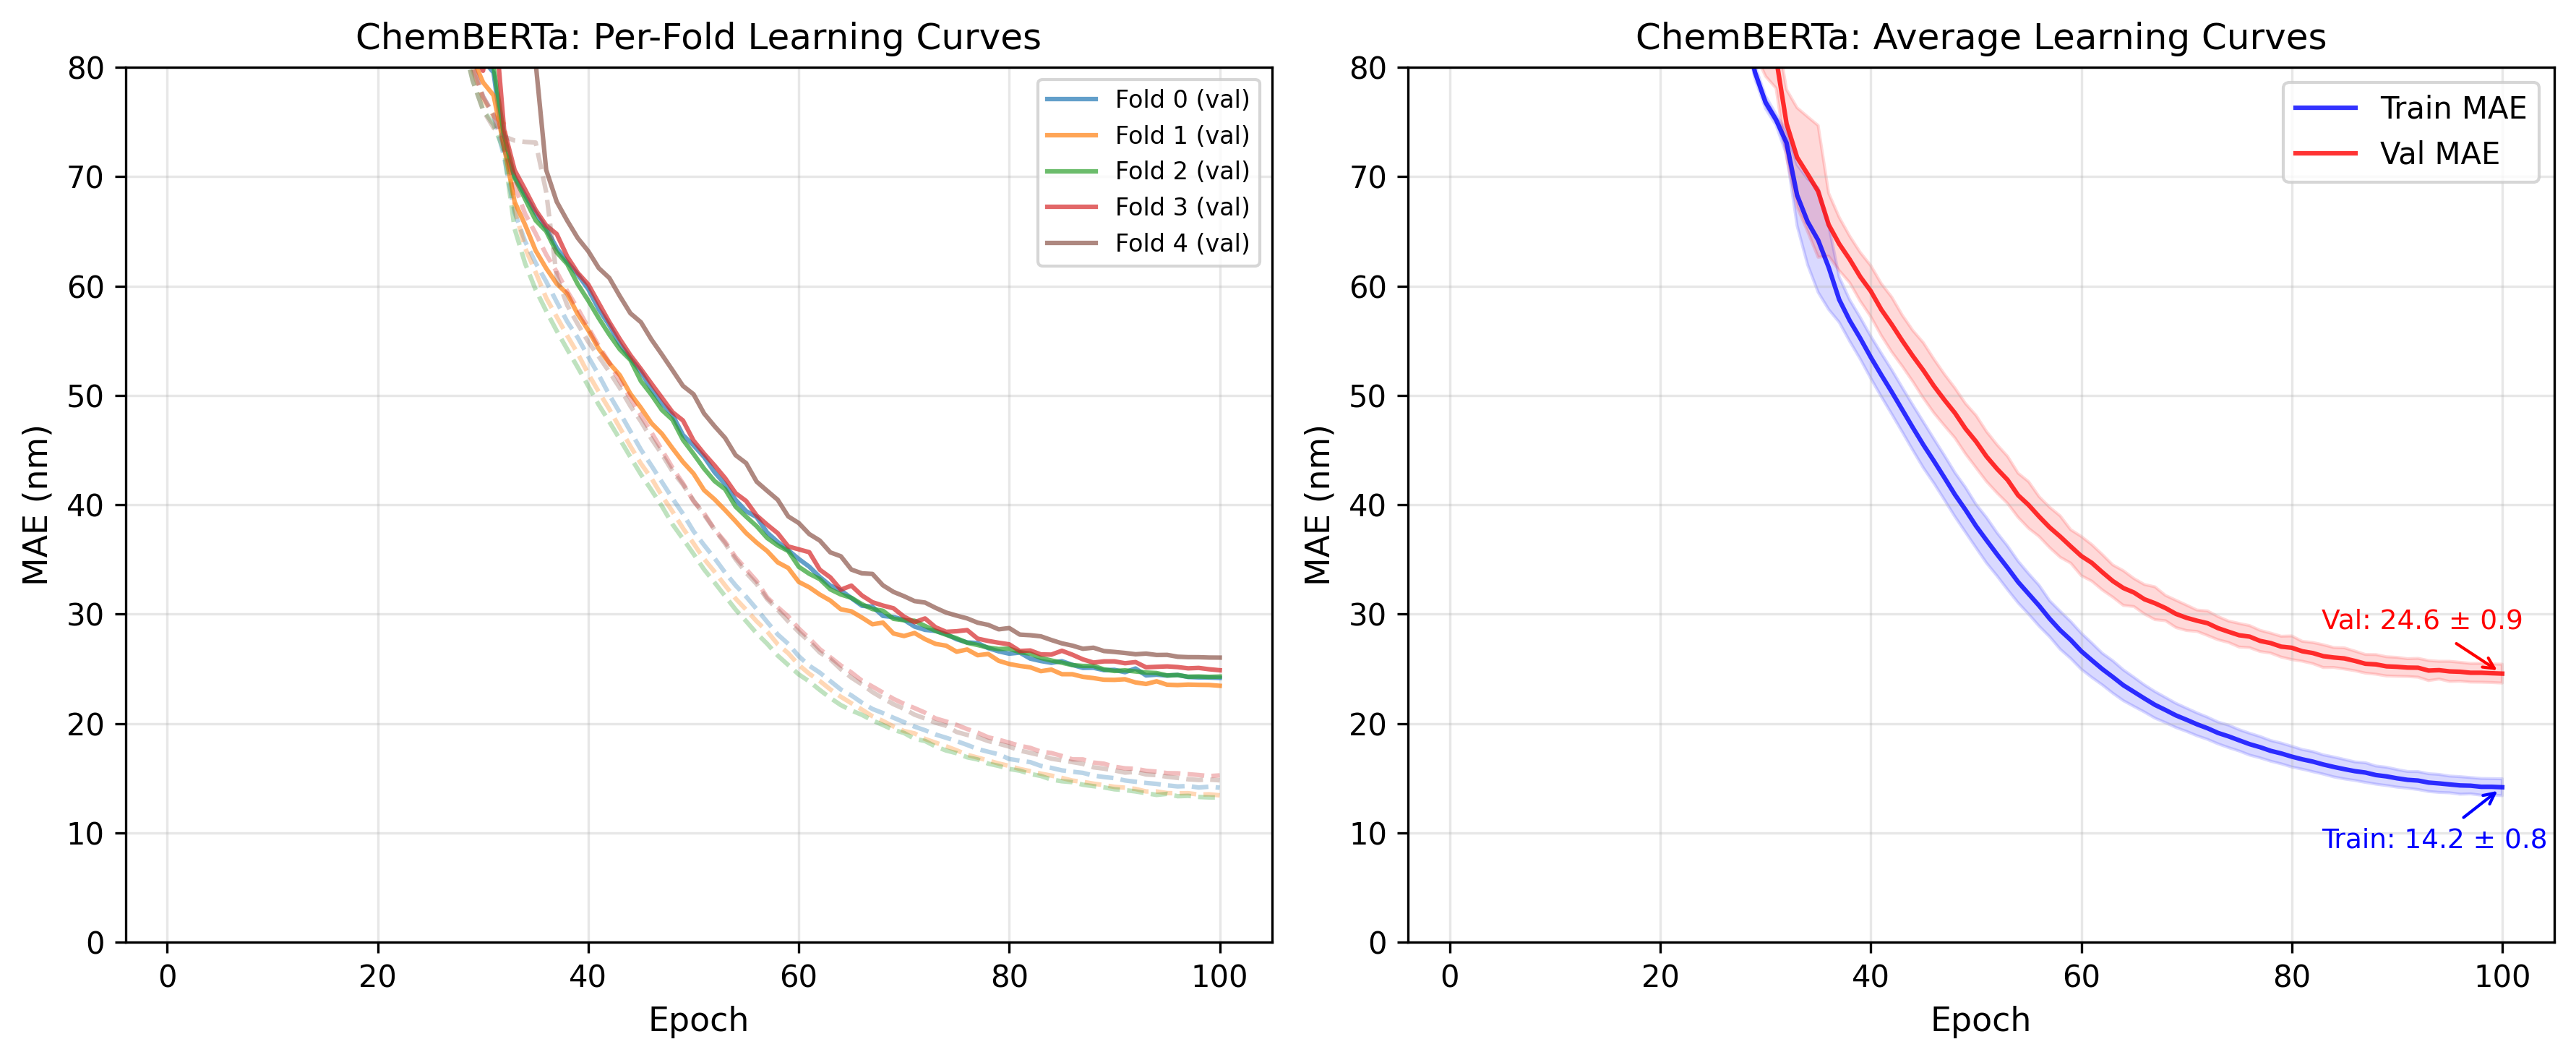
\includegraphics[width=\textwidth]{results/chemberta_learning_curves.png}
    \caption{ChemBERTa fine-tuning learning curves. Left: per-fold validation MAE (solid) and training MAE (dashed). Right: mean $\pm$ 1 standard deviation across folds, with final values annotated.}
    \label{fig:chemberta_curves}
\end{figure}


\section{Hyperparameter Tuning Asymmetry}
\label{sec:tuning_asymmetry}

Table~\ref{tab:tuning_asymmetry} compares the effect of hyperparameter tuning for both RF and BiGRU, demonstrating that the in-distribution performance gap between model families is not an artifact of asymmetric tuning effort.

\begin{table}[htbp]
\centering
\caption{Effect of hyperparameter tuning on cross-validated performance (stratified 5-fold CV).}
\label{tab:tuning_asymmetry}
\begin{tabular}{lccc}
\toprule
\textbf{Model} & \textbf{RMSE (nm)} & \textbf{MAE (nm)} & \textbf{Improvement} \\
\midrule
RF (default, $\sqrt{d}$)         & 32.18 $\pm$ 1.74 & 15.42 $\pm$ 0.47 & --- \\
RF (tuned, $0.3d$)               & 31.34 $\pm$ 1.82 & 15.16 $\pm$ 0.44 & $-$2.6\% RMSE \\
\midrule
BiGRU (default, 2L/128u)         & 36.45 $\pm$ 1.12 & 20.70 $\pm$ 0.51 & --- \\
BiGRU (tuned, 3L/256u) & 34.71 $\pm$ 1.40 & 18.09 $\pm$ 0.59 & $-$4.8\% RMSE \\
\bottomrule
\end{tabular}
\end{table}

BiGRU HPO was conducted using Optuna TPE (25 trials on fold~0), with the best configuration extended to full 5-fold cross-validation, yielding a 4.8\% RMSE improvement over the default architecture.
Even the default RF (RMSE = 32.18~nm) outperforms the tuned BiGRU (RMSE = 34.71~nm), while RF tuning provides only an additional 2.6\% improvement.
BiGRU tuning narrows the gap from 14\% to 10\%, but the remaining difference suggests that the fingerprint representation has an inherent advantage for in-distribution UV absorption prediction.
ChemBERTa hyperparameters were not tuned due to the prohibitive training cost ($\sim$3 hours per fold for 44.1M parameters).


\section{SMARTS Rules and Metrics for Non-Local Subset Analysis}
\label{si:nonlocal_smarts}

The non-local subset analysis reported in main-text Section~\ref{sec:nonlocal_subsets} and Table~\ref{tab:nonlocal_subsets} uses the SMARTS patterns listed in Tables~\ref{tab:si_donor_smarts}--\ref{tab:si_motif_smarts}.

\textit{Donors} are lone-pair-bearing substituents on an aromatic carbon that push electron density into the $\pi$ system. The amide nitrogen is explicitly excluded (\texttt{!\$(N-C=O)}) because the acyl group converts the nitrogen into a weak acceptor rather than a donor.
\textit{Acceptors} are strongly electron-withdrawing substituents on a conjugated $sp^2$ centre---aromatic carbon (\texttt{[c]}) or an $sp^2$ alkene carbon (\texttt{[CX3](=[\#6,\#7])[!\#1]}). The alkene branch is included so that push--pull cinnamic acids such as ferulic acid (\texttt{COc1cc(/C=C/C(=O)O)ccc1O}) are correctly captured as donor--acceptor compounds.
The donor-count column shows the number of distinct atom-set matches per molecule (using RDKit's \texttt{GetSubstructMatches} with \texttt{uniquify=True}); a molecule with two methoxy groups on the same ring contributes a donor count of 2 to the D-A-D rule.

\begin{table}[htbp]
\centering
\caption{Donor SMARTS patterns used to identify D-A and D-A-D molecules.}
\label{tab:si_donor_smarts}
\small
\begin{tabular}{lll}
\toprule
\textbf{Rule name} & \textbf{SMARTS} & \textbf{Matches} \\
\midrule
aryl\_NH2  & \verb|[c]-[NX3;H2;!$(N(C=O));!$(N-N=O)]|                       & primary aryl amine \\
aryl\_NHR  & \verb|[c]-[NX3;H1;!$(N-C=O);!$(N-N=O);!$(N-S(=O))]|            & secondary aryl amine (non-amide) \\
aryl\_NR2  & \verb|[c]-[NX3;H0;!$(N-C=O);!$(N-N=O);!$(N-S(=O))]([#6])[#6]|  & tertiary aryl amine \\
aryl\_OH   & \verb|[c]-[OX2H1]|                                              & aryl hydroxyl \\
aryl\_OR   & \verb|[c]-[OX2;H0]-[CX4]|                                       & aryl ether/methoxy \\
aryl\_SH   & \verb|[c]-[SX2H1]|                                              & aryl thiol \\
aryl\_SR   & \verb|[c]-[SX2;H0]-[CX4]|                                       & aryl sulfide \\
\bottomrule
\end{tabular}
\end{table}

\begin{table}[htbp]
\centering
\caption{Acceptor SMARTS patterns. The \emph{sp$^2$-anchor} \texttt{[\$([c]),\$([CX3](=[\#6,\#7])[!\#1])]} matches either an aromatic carbon or an alkene/imine sp$^2$ carbon so that push--pull cinnamic-acid-type acceptors are detected.}
\label{tab:si_acceptor_smarts}
\small
\begin{tabular}{lll}
\toprule
\textbf{Rule name} & \textbf{SMARTS} & \textbf{Matches} \\
\midrule
nitro          & \verb|sp2-[$([NX3+](=O)[O-]),$([NX3](=O)=O)]|  & nitro \\
CN             & \verb|sp2-[CX2]#[NX1]|                          & cyano / nitrile \\
CHO            & \verb|sp2-[CX3H1](=O)|                          & aldehyde \\
ketone         & \verb|sp2-[CX3](=O)[#6]|                        & ketone \\
COOH           & \verb|sp2-[CX3](=O)[OX2H1]|                     & carboxylic acid \\
COOR           & \verb|sp2-[CX3](=O)[OX2H0][#6]|                 & ester \\
amide          & \verb|sp2-[CX3](=O)[NX3]|                       & amide \\
SO2            & \verb|sp2-[SX4](=O)(=O)|                        & sulfonyl \\
CF3            & \verb|sp2-[CX4](F)(F)F|                         & trifluoromethyl \\
aromatic\_N+   & \verb|[c][n+,N+;X3]|                            & pyridinium / acridinium \\
dicyanovinyl   & \verb|[#6]=C([CX2]#[NX1])[CX2]#[NX1]|           & dicyanovinyl \\
malononitrile  & \verb|[CX4H1]([CX2]#N)[CX2]#N|                  & malononitrile \\
\bottomrule
\end{tabular}
\end{table}

\begin{table}[htbp]
\centering
\caption{Specific dye motifs.}
\label{tab:si_motif_smarts}
\small
\begin{tabular}{lll}
\toprule
\textbf{Rule name} & \textbf{SMARTS} & \textbf{Matches} \\
\midrule
azo       & \verb|[c]-[N;X2]=[N;X2]-[c]|                                                            & aryl azo bridge \\
bodipy    & \verb|[B](F)(F)([#7;R])[#7;R]|                                                          & BF$_2$ bonded to two ring nitrogens \\
cyanine   & \verb|[NX3,nX3]-,=[CX3]=,-[CX3]-,=[CX3]=,-[CX3]-,=[NX3+,nX3+]|                          & open-chain polymethine cyanine \\
squaraine & \verb|C1(=O)C(=*)C(=O)C1=*|                                                             & squaric-acid-derived push--pull \\
stilbene  & \verb|[c]-[CH]=[CH]-[c]|                                                                & 1,2-diarylethene scaffold \\
\bottomrule
\end{tabular}
\end{table}

\begin{table}[htbp]
\centering
\caption{Non-local subset sizes in the full Joung+Beard primary dataset ($n_{\text{total}} = 18{,}755$). Subset definitions are unioned with each test fold to obtain the per-fold $n$ values reported in main-text Table~\ref{tab:nonlocal_subsets}.}
\label{tab:si_subset_counts}
\small
\begin{tabular}{lrr}
\toprule
\textbf{Subset} & $n$ & \textbf{\% of dataset} \\
\midrule
Full dataset                 & 18{,}755 & 100.00 \\
$\lambda_{\max} > 500$~nm    &  3{,}887 &  20.73 \\
$\lambda_{\max} > 600$~nm    &  1{,}573 &   8.39 \\
Azo (Ar--N$=$N--Ar)          &     264  &   1.41 \\
D-A                          &  6{,}059 &  32.31 \\
D-A-D                        &  2{,}188 &  11.67 \\
BODIPY core                  &  1{,}766 &   9.42 \\
Cyanine                      &      59  &   0.31 \\
Stilbene                     &  1{,}537 &   8.20 \\
Squaraine                    &       0  &   0.00 \\
\midrule
Union (any non-local)        &  9{,}229 &  49.21 \\
\bottomrule
\end{tabular}
\end{table}

\begin{table}[htbp]
\centering
\caption{Full per-model error breakdown on the non-local subsets (mean $\pm$ std over the five stratified test folds). Best result per metric per subset in bold. The Squaraine subset is empty in the Joung+Beard dataset and is omitted. Reproduced via \texttt{python3 analyze\_nonlocal\_subsets.py --models rf\_tuned xgboost\_v2 chemprop\_v2 bigru\_tuned chemberta --regen\_xgboost}.}
\label{tab:si_nonlocal_full}
\scriptsize
\setlength{\tabcolsep}{3pt}
\begin{tabular}{lcccccc}
\toprule
\textbf{Subset / metric} & $n$ & \textbf{RF} & \textbf{Chemprop} & \textbf{BiGRU} & \textbf{ChemBERTa} & \textbf{XGBoost} \\
\midrule
\multicolumn{7}{l}{\textbf{RMSE (nm)}} \\
Full dataset      & 3751 & \textbf{31.34 $\pm$ 2.04} & 31.69 $\pm$ 3.56  & 34.71 $\pm$ 1.57  & 50.39 $\pm$ 2.57  & 33.72 $\pm$ 1.77 \\
$\lambda > 500$   &  777 & 51.95 $\pm$ 5.25 & \textbf{45.31 $\pm$ 7.72} & 52.48 $\pm$ 5.90 & 98.42 $\pm$ 6.13 & 51.31 $\pm$ 5.32 \\
$\lambda > 600$   &  315 & 69.47 $\pm$ 9.26 & \textbf{60.89 $\pm$ 15.20} & 69.64 $\pm$ 10.78 & 148.18 $\pm$ 10.01 & 67.82 $\pm$ 9.33 \\
Azo               &   53 & 32.63 $\pm$ 7.65 & \textbf{29.18 $\pm$ 4.35} & 38.85 $\pm$ 6.28 & 37.27 $\pm$ 4.33 & 34.29 $\pm$ 6.08 \\
D-A               & 1212 & 24.31 $\pm$ 0.72 & \textbf{23.05 $\pm$ 2.67} & 28.14 $\pm$ 1.00 & 43.74 $\pm$ 1.61 & 26.96 $\pm$ 0.91 \\
D-A-D             &  438 & 26.44 $\pm$ 2.71 & \textbf{24.05 $\pm$ 1.54} & 30.85 $\pm$ 2.65 & 39.48 $\pm$ 1.32 & 28.65 $\pm$ 2.77 \\
BODIPY            &  353 & \textbf{22.25 $\pm$ 4.28} & \textbf{22.36 $\pm$ 1.91} & 27.23 $\pm$ 5.49 & 69.75 $\pm$ 8.28 & 24.70 $\pm$ 2.88 \\
Cyanine           &   12 & \textbf{16.55 $\pm$ 4.96} & 30.93 $\pm$ 4.35 & 17.87 $\pm$ 7.68 & 33.62 $\pm$ 6.86 & 27.67 $\pm$ 8.75 \\
Stilbene          &  307 & \textbf{27.76 $\pm$ 3.85} & 28.79 $\pm$ 5.51 & 34.52 $\pm$ 4.35 & 45.77 $\pm$ 5.58 & 32.21 $\pm$ 3.57 \\
Non-local union   & 1846 & 36.76 $\pm$ 3.03 & \textbf{33.47 $\pm$ 4.75} & 38.96 $\pm$ 3.26 & 66.10 $\pm$ 3.63 & 37.72 $\pm$ 2.90 \\
\midrule
\multicolumn{7}{l}{\textbf{MAE (nm)}} \\
Full dataset      & 3751 & \textbf{15.16 $\pm$ 0.50} & 16.84 $\pm$ 1.94 & 18.09 $\pm$ 0.65 & 24.31 $\pm$ 1.16 & 20.06 $\pm$ 0.53 \\
$\lambda > 500$   &  777 & 25.16 $\pm$ 1.88 & \textbf{22.26 $\pm$ 3.06} & 26.56 $\pm$ 2.44 & 64.90 $\pm$ 4.81 & 28.34 $\pm$ 2.28 \\
$\lambda > 600$   &  315 & 35.40 $\pm$ 4.34 & \textbf{29.00 $\pm$ 5.76} & 36.02 $\pm$ 5.16 & 128.49 $\pm$ 9.58 & 37.34 $\pm$ 4.31 \\
Azo               &   53 & 21.24 $\pm$ 4.47 & \textbf{19.80 $\pm$ 2.07} & 26.44 $\pm$ 3.96 & 23.02 $\pm$ 1.76 & 24.48 $\pm$ 2.20 \\
D-A               & 1212 & \textbf{12.58 $\pm$ 0.43} & 14.44 $\pm$ 1.94 & 15.38 $\pm$ 0.44 & 21.27 $\pm$ 0.51 & 17.46 $\pm$ 0.33 \\
D-A-D             &  438 & \textbf{14.47 $\pm$ 0.93} & 15.30 $\pm$ 1.62 & 17.63 $\pm$ 0.69 & 21.10 $\pm$ 1.13 & 18.91 $\pm$ 1.46 \\
BODIPY            &  353 & \textbf{10.25 $\pm$ 0.97} & 13.53 $\pm$ 1.74 & 15.22 $\pm$ 2.43 & 42.90 $\pm$ 5.07 & 15.48 $\pm$ 1.80 \\
Cyanine           &   12 & \textbf{13.13 $\pm$ 4.05} & 25.36 $\pm$ 5.09 & 15.06 $\pm$ 6.68 & 25.12 $\pm$ 7.78 & 24.19 $\pm$ 6.98 \\
Stilbene          &  307 & \textbf{15.53 $\pm$ 1.48} & 18.53 $\pm$ 3.38 & 18.90 $\pm$ 1.42 & 25.25 $\pm$ 2.62 & 21.57 $\pm$ 1.44 \\
Non-local union   & 1846 & \textbf{16.74 $\pm$ 0.63} & 17.15 $\pm$ 2.15 & 19.33 $\pm$ 0.94 & 34.32 $\pm$ 1.78 & 21.11 $\pm$ 0.73 \\
\midrule
\multicolumn{7}{l}{$\boldsymbol{R^2}$} \\
Full dataset      & 3751 & \textbf{0.914 $\pm$ 0.011} & 0.911 $\pm$ 0.018 & 0.894 $\pm$ 0.010 & 0.777 $\pm$ 0.021 & 0.900 $\pm$ 0.010 \\
$\lambda > 500$   &  777 & 0.597 $\pm$ 0.072 & \textbf{0.690 $\pm$ 0.092} & 0.588 $\pm$ 0.079 & $-0.439 \pm 0.138$ & 0.607 $\pm$ 0.072 \\
$\lambda > 600$   &  315 & $-0.134 \pm 0.219$ & \textbf{0.105 $\pm$ 0.362} & $-0.144 \pm 0.276$ & $-4.142 \pm 0.395$ & $-0.082 \pm 0.222$ \\
Azo               &   53 & 0.702 $\pm$ 0.108 & \textbf{0.763 $\pm$ 0.054} & 0.580 $\pm$ 0.097 & 0.616 $\pm$ 0.046 & 0.674 $\pm$ 0.079 \\
D-A               & 1212 & 0.938 $\pm$ 0.002 & \textbf{0.944 $\pm$ 0.012} & 0.917 $\pm$ 0.005 & 0.798 $\pm$ 0.018 & 0.923 $\pm$ 0.005 \\
D-A-D             &  438 & 0.919 $\pm$ 0.019 & \textbf{0.934 $\pm$ 0.005} & 0.890 $\pm$ 0.023 & 0.820 $\pm$ 0.020 & 0.905 $\pm$ 0.021 \\
BODIPY            &  353 & \textbf{0.936 $\pm$ 0.020} & \textbf{0.936 $\pm$ 0.010} & 0.905 $\pm$ 0.029 & 0.379 $\pm$ 0.079 & 0.922 $\pm$ 0.013 \\
Cyanine           &   12 & \textbf{0.865 $\pm$ 0.088} & 0.544 $\pm$ 0.180 & 0.848 $\pm$ 0.095 & 0.436 $\pm$ 0.291 & 0.618 $\pm$ 0.284 \\
Stilbene          &  307 & \textbf{0.916 $\pm$ 0.018} & 0.909 $\pm$ 0.027 & 0.870 $\pm$ 0.023 & 0.771 $\pm$ 0.044 & 0.887 $\pm$ 0.019 \\
Non-local union   & 1846 & 0.904 $\pm$ 0.014 & \textbf{0.920 $\pm$ 0.020} & 0.892 $\pm$ 0.016 & 0.690 $\pm$ 0.027 & 0.899 $\pm$ 0.014 \\
\bottomrule
\end{tabular}
\end{table}

A few additional observations that did not fit in the main text:
(i) The MAE column reinforces the RMSE story for the long-wavelength subsets ($\lambda > 500$ and $\lambda > 600$~nm: Chemprop best on both metrics) but flips on the local-context subsets (D-A, D-A-D, BODIPY, Stilbene, Cyanine: RF lowest MAE despite being tied or slightly behind on RMSE). This is consistent with RF's residuals being concentrated near zero with a longer tail of larger errors, while Chemprop produces a more uniformly spread residual distribution---squared-error metrics weight the tail more heavily.
(ii) The cyanine subset contains only $\sim$12 test molecules per fold, so its metrics carry large fold-to-fold variance and should not be read as a reliable model ranking.
(iii) ChemBERTa's $R^2 = -4.14$ on the $\lambda > 600$~nm subset reflects the prediction-ceiling artefact discussed in Section~\ref{sec:error_analysis} of the main text---ChemBERTa is essentially predicting a constant in this region, so the variance-explained metric goes strongly negative.


\section{BiGRU Character-Type Saliency}
\label{sec:chartype_saliency}

Figure~\ref{fig:bigru_chartype} shows the mean gradient saliency aggregated by SMILES character type across all wetlab validation molecules.
Bond symbols (\texttt{=}, \texttt{\#}) receive the highest mean saliency, reflecting the critical role of double and triple bonds in establishing conjugated $\pi$-systems that determine UV absorption.
Heteroatoms (N, O, S) rank second, consistent with their role as electron donors and acceptors in chromophores, while aromatic atom characters and aliphatic carbons receive lower saliency, and brackets/syntax characters contribute minimally.

\begin{figure}[htbp]
    \centering
    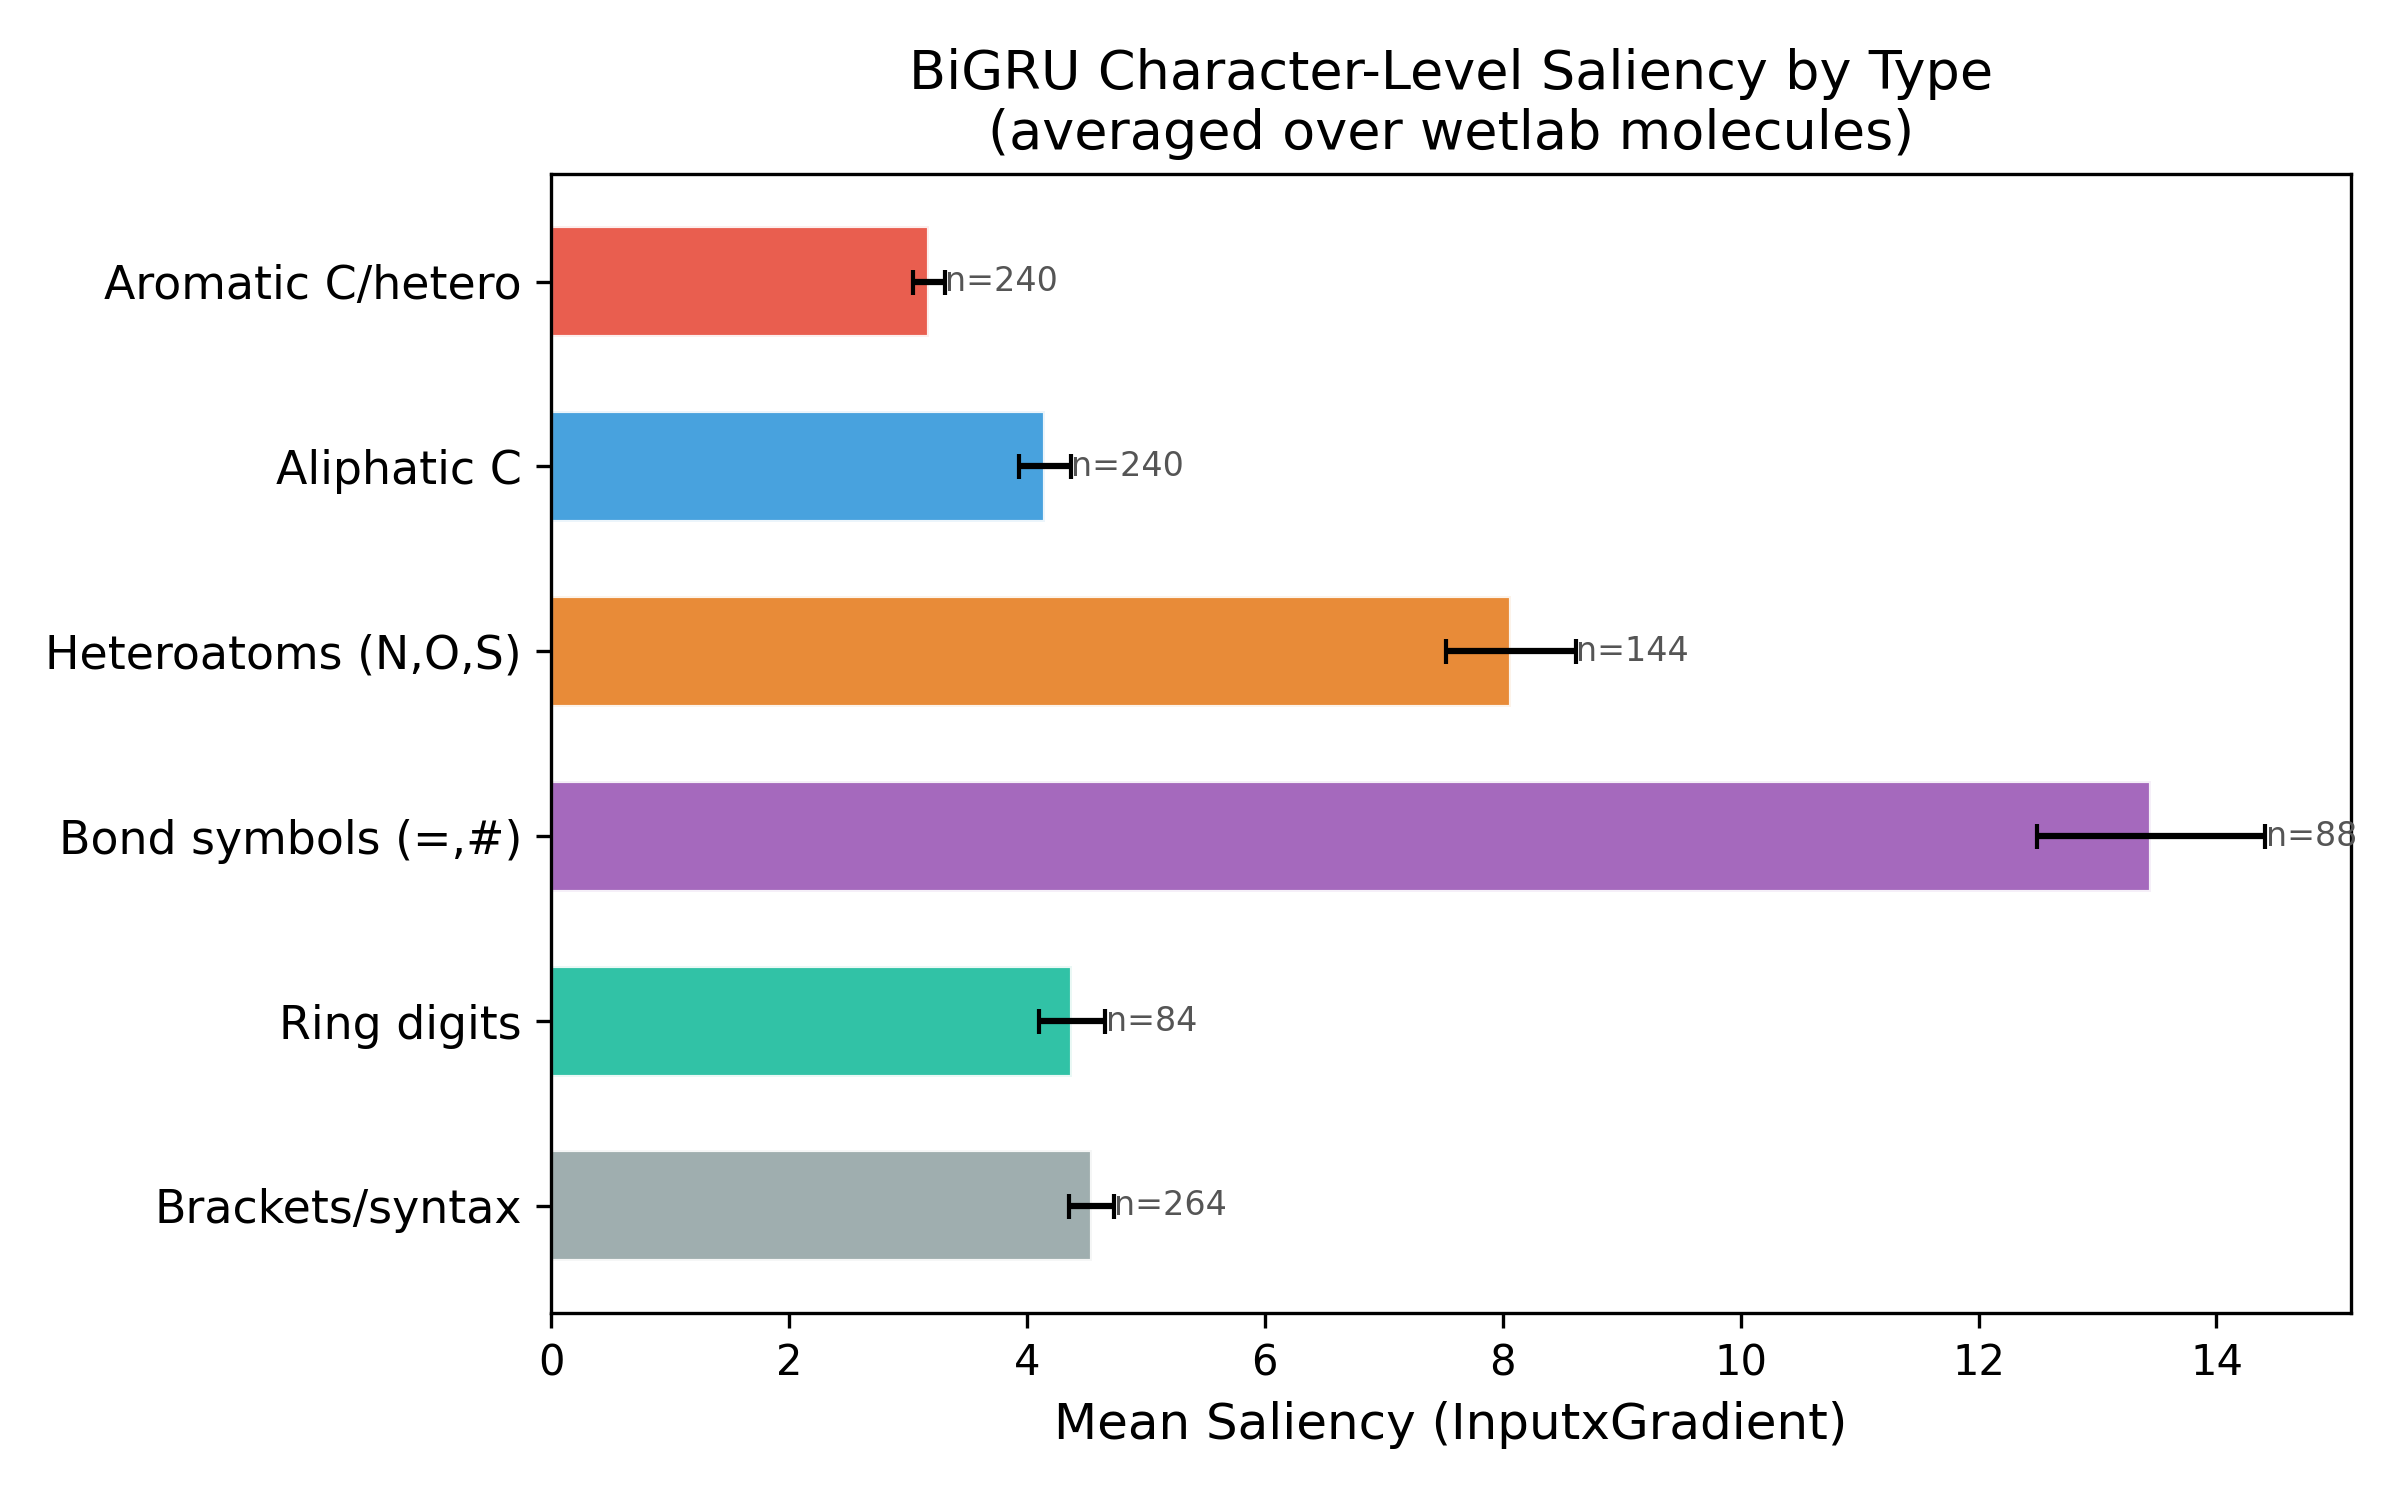
\includegraphics[width=0.65\textwidth]{results/bigru_saliency_chartype.png}
    \caption{Mean BiGRU gradient saliency by SMILES character type, averaged over all wetlab validation molecules. Bond symbols (\texttt{=}, \texttt{\#}) and heteroatoms receive the highest saliency, consistent with the role of conjugated $\pi$-systems and electron-donating/withdrawing groups in determining UV absorption.}
    \label{fig:bigru_chartype}
\end{figure}

\end{document}
